% summary.tex -- what the neuro results say, and what to check before submission.
% Standalone: pdflatex summary.tex. Figures/tables are referenced by relative
% path, so run it from paper_results/.
\documentclass[11pt]{article}
\usepackage[margin=1in]{geometry}
\usepackage{booktabs,graphicx,amsmath,microtype}
\usepackage[colorlinks=true,allcolors=blue]{hyperref}
\graphicspath{{figures/supplementary/}}
\title{Brain--model alignment across development: summary of results}
\author{}
\date{}

\begin{document}
\maketitle

\section{The main result, in one paragraph}

Across 29 model families, four linguistic domains, three neuroimaging studies
and 16 log-spaced training-token bins, brain--model representational alignment
is small in absolute terms ($|\bar\rho| < 0.03$ everywhere) and, critically,
\emph{does not have one shape}. More training data strengthens alignment in
grammar, reverses it in semantics and plausibility, and leaves phonology
indistinguishable from noise throughout. Behaviour moves in the opposite
direction from alignment where the two can be compared: minimal-pair accuracy
rises with training in three of four domains, and in plausibility it is
\emph{anticorrelated} with alignment at $\rho = -0.64$. The developmental
analogy the paper sets up---LM training checkpoint stands in for child
age---therefore holds for behaviour and fails for representation.

\section{Main text: Section 5}

\paragraph{Brain alignment (\S5.1).} Grammar is the only domain positive and
zero-excluding in every occupied token bin, peaking at $\bar\rho = 0.0253$ and
settling at $0.0115$. Plausibility starts positive ($0.0152$) and crosses into
negative, zero-excluding values from intermediate training onward, ending at
$-0.0076$. Semantics follows the same reversal more weakly. Phonology reaches
no positive zero-excluding bin.

\paragraph{Behaviour (\S5.2).} Children improve monotonically with age in
every domain (e.g.\ grammar $0.718 \to 0.839$ from age 5 to 9). Models improve
with tokens in three domains---plausibility $0.471 \to 0.913$, grammar
$0.482 \to 0.720$, semantics $0.506 \to 0.685$---but phonology stays within
$\pm 0.05$ of chance across all 15 occupied bins.

\paragraph{Measure relationships (\S5.3).} Of 20 domain\,$\times$\,pair
Spearman correlations, 19 are weak ($|\rho| \le 0.21$), including every
correlation involving mechanistic sparsity or circuit selectivity. The
exception is plausibility accuracy against plausibility alignment,
$\rho = -0.641$.

\section{What the supplementary figures add}

Section 5 pools across dataset, child age, model family and architecture. The
nine supplementary figures (\texttt{figures/supplementary/}) open those axes;
Table~\ref{tab:new} lists the results that pooling hid.

\begin{table}[h]
\centering\small
\begin{tabular}{@{}llp{7.4cm}@{}}
\toprule
& Axis opened & Result \\
\midrule
S1 & child age band & Age matters, but at age 9---the one band two datasets
share---the \emph{dataset} drives the difference, not the age. \\
S2 & the noise ceiling & Ceilings run $0.235$--$0.881$. Normalised,
phonology reaches $\sim$7\% of ceiling at $10^{10}$ tokens, its strongest
showing anywhere. \\
S3, S4 & anatomical mask & Grammar's alignment is \textbf{anatomically
graded}: $+0.0153$ whole-brain, $+0.0135$ auditory, $+0.0091$ motor,
$+0.0041$ under the phonology mask, with non-overlapping CIs. The other three
domains do not move. \\
S5 & the $\rho=-0.641$ entry & Reproduces at $-0.639$ and is the only visible
structure across the four panels. \\
S6 & scale and architecture & Scale does nothing. At matched seeds,
\textbf{Pythia's grammatical alignment is $+0.0281$ against mamba's $+0.0058$
and rwkv's $+0.0106$}---a 3--5$\times$ architecture effect inside a result
reported as uniformly tiny. \\
S7 & brain- vs.\ model-side localisation & The two localisation measures sit
in different ranges and neither tracks the other. \\
S8 & network depth & Grammar, semantics and plausibility circuits migrate
from $\sim$0.46 to 0.62--0.71 relative depth over training;
\textbf{phonology alone does not move} ($0.491 \to 0.457$). \\
S9 & the fourth study & ds001894, plus a coverage map of both alignment runs. \\
\bottomrule
\end{tabular}
\caption{New results, by the axis the main text pools over.}
\label{tab:new}
\end{table}

Two of these sharpen the paper's own story. Phonology is the domain that never
aligns (\S5.1) \emph{and} never leaves chance behaviourally (\S5.2)---S8 adds
that it is also the one domain whose circuit never moves in depth. And the
grammar effect, the paper's single robust positive, turns out to depend on
where in the brain one looks and on which architecture one trains.

\begin{figure}[h]
\centering
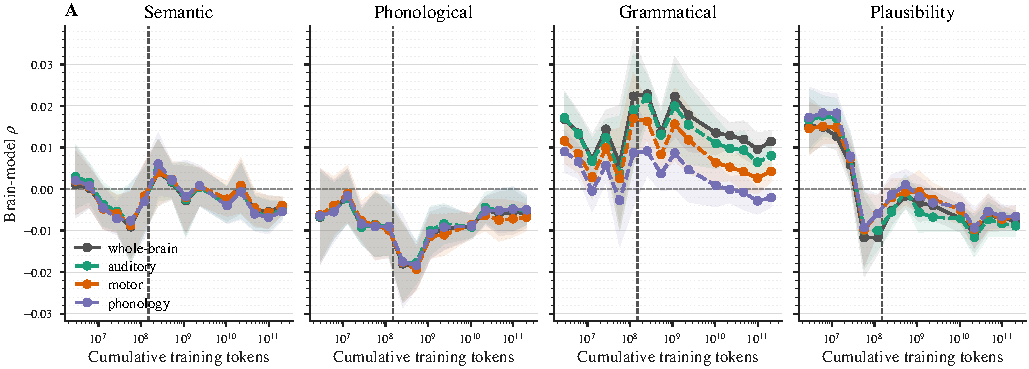
\includegraphics[width=\linewidth]{figS4_roi_trajectories.pdf}
\caption{Alignment under each anatomical mask. Grammar (third panel)
separates by mask; the other three domains do not.}
\end{figure}

\section{Publishable tables}

\texttt{tables/} holds eight booktabs tables, each with the CSV it was built
from: T1 alignment by domain (a recomputation of Table~2), T2 measure
correlations (Table~5), T3 domain\,$\times$\,mask, T4 architecture at matched
seeds, T5 age band\,$\times$\,dataset, T6 circuit depth, T7 study coverage,
T8 noise ceilings.

\section{Three things to settle before submission}

\paragraph{1. Table 2's phonology row does not reconcile.} It reports no token
bin with a positive zero-excluding CI and a last-bin mean of $+0.0044$.
Recomputing from \texttt{results/alignment\_rows.csv} reproduces plausibility
exactly (4/9/2), grammar to within one bin (14/0/1 vs.\ 15/0/0) and semantics
closely (5/3/7 vs.\ 7/3/5)---but gives phonology 6/5/4 at $+0.0079$. The sign
pattern differs, and no subset of the three datasets reproduces the submitted
row. \S6.1's claim that phonology never reaches a positive zero-excluding bin
rests on it.

\paragraph{2. The unit of the confidence interval.} A checkpoint contributes
one row per (dataset, domain, session) cell, so treating rows as independent
inflates $n$ by up to $8\times$. Every supplementary figure and table averages
within checkpoint first, which is also what reproduces Table~4's $n=30$ in the
last bin. If the main text's intervals were taken over raw rows they are too
narrow.

\paragraph{3. All four studies fail the positive-control gate.} ds001894
(0/16 stimulus tests significant), ds002236 (0/30), ds003604 (0/108) and
ds006239 (0/38) all fail. Nothing stimulus-driven correlates with the brain
RDMs, so every alignment number is bounded by an instrument that has not been
shown to work. This is documented per dataset in
\texttt{paper\_results/ds*/README.md} and belongs in the limitations section.

\paragraph{Coverage.} All four studies are used, but no single alignment run
covers all four: ds001894 is ``not run'' in the 29-family grid
(\texttt{results/coverage\_matrix.csv}) and appears via the 15-family devai
grid (S9) and the brain-side localisation (S7). The two runs share three
studies and nine model families and disagree by up to $0.067$ where they
overlap---wider than the entire effect range reported---so they are never
pooled. Bringing ds001894 into the main results requires running the
29-family grid on it.

\section{Reproducing}

\begin{verbatim}
python scripts/make_supplementary_figures.py   # S1-S9 -> figures/supplementary/
python scripts/make_supplementary_tables.py    # T1-T8 -> tables/
\end{verbatim}

Both run offline. Shared loaders and the CI convention are in
\texttt{scripts/figlib.py}; the plot style is vendored verbatim from
beetle-analyze-meco as \texttt{src/viz/plot\_style.py}; the anatomical
rendering is \texttt{src/viz/brainplot.py}, whose docstring explains why these
are mask definitions tinted by a measured scalar and not per-voxel maps.

\end{document}
